\section{Audit Decisions, Recovery, and Strong Baselines}
\label{sec:recovery-results}

\subsection{RQ3: What Does ICBA Authorize?}
Direct unshifted reuse fails every candidate certificate in the original refresh replay and routes all 20 targets to the endpoint. ICBA therefore blocks uncertified efficiency without manufacturing a saving. TCP changes the candidate before certification. The original allocation accepts 19/20 candidates; the $0.025+0.025$ sensitivity accepts all ten SIFT and six Arxiv candidates, with four certified endpoint fallbacks and no abstention.

\begin{figure*}[t]
\centering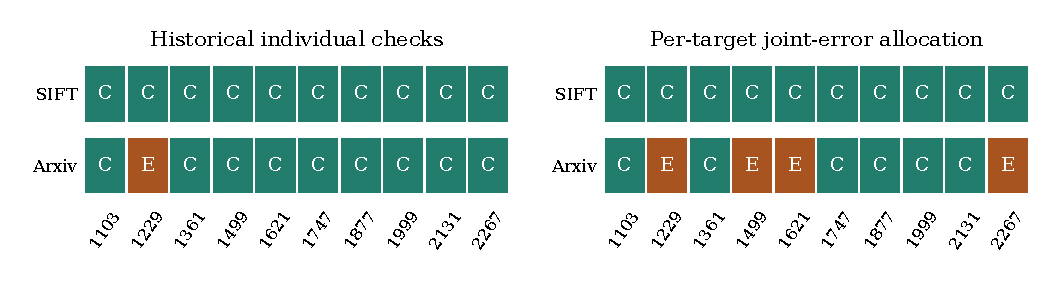
\includegraphics[width=\textwidth]{figures_v3/decisions.pdf}
\caption{Completed target decisions. C denotes candidate and E endpoint fallback. The left procedure uses historical individual $0.05/0.05$ checks and does not provide 95\% joint control for the completed choice. The right allocates $0.025/0.025$ per target, changing Arxiv composition from nine to six candidates.}
\label{fig:decisions}
\Description{SIFT accepts ten candidates under both rules. Arxiv accepts nine under the original allocation and six under the stricter allocation.}
\end{figure*}

\subsection{RQ4a: Endpoint-Relative Recovery and Incremental Value}
TCP's original completed decisions reduce mean NDC by 44.39\% on SIFT and 44.79\% on Arxiv. Under the joint-error allocation, SIFT is unchanged and Arxiv retains 29.86 [14.75,45.00]\%. Risk is 1.79\% and 1.68\%, respectively. Both remain positive relative to each target's endpoint.

The equal-information comparison asks the stronger question. It is a post-hoc frozen-response sensitivity, not a preregistered confirmation. Against target-global calibration with the same 500 selection, 500 certification, and 1,000 evaluation queries, TCP gains a further 27.60 [17.92, 36.72]\% mean NDC on SIFT. Arxiv's gain is 10.78 [$-8.48$, 29.43]\%, while its p95 ratio is 1.109 [1.012, 1.285]. Query conditioning therefore adds resolved value only on SIFT under the registered event, grid, and SLA.

\begin{figure}[t]
\centering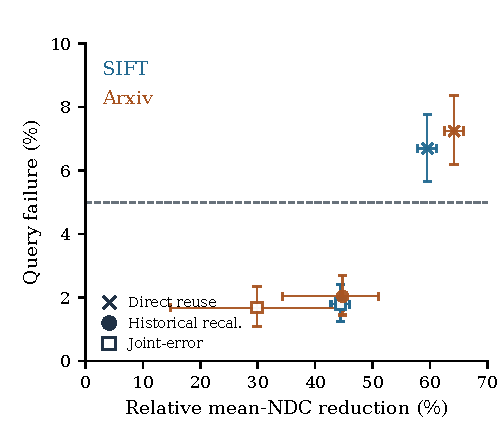
\includegraphics[width=\linewidth]{figures_v3/tradeoff.pdf}
\caption{Refresh risk--work tradeoff with crossed 95\% intervals. Marker shapes denote direct reuse ($\times$), historical recalibration ($\circ$), and the joint-error completed decision ($\square$); color denotes dataset. The endpoint is the zero-gain reference and is not plotted.}
\label{fig:tradeoff}
\Description{Direct reuse has high failure. Target-recalibrated policies have lower risk and retain positive search-work savings.}
\end{figure}

\subsection{RQ4b: Prospective Build Confirmation}
\label{sec:prospective}
\label{sec:fresh-bridge}
The prospective confirmation freezes source one-rung before eight new insertion-permutation builds and three new query roles per dataset are accessed. All 56 directed decisions per dataset accept the candidate, with zero fallback or abstention (Table~\ref{tab:s9-prospective}). Across 144,000 response cells and 112,000 raw timing measurements, native and measured top-$k$ agree exactly. Mean candidate/endpoint latency is 0.280/0.576 ms on SIFT and 1.161/1.662 ms on Arxiv. Sparse-grid and 2.5\%-risk sensitivities remain qualified but collapse to the endpoint, defining preregistered boundaries rather than failures of the primary configuration.

\begin{table*}[t]
\caption{Prospective confirmation on eight new target builds per dataset. C/F/A counts candidate/fallback/abstention. Risk and wall-time reduction are percentages [95\% crossed target-build/query interval]. p95 is the completed-decision/endpoint wall-time ratio [95\% interval]; LOTO is minimum wall-time reduction after deleting one target.}
\label{tab:s9-prospective}
\small\begin{tabular*}{\textwidth}{@{\extracolsep{\fill}}lrrrrr@{}}\toprule
Dataset & C/F/A & Eval. risk & Wall-time reduction & p95 ratio & LOTO reduction\\\midrule
\SProspectiveRows
\bottomrule\end{tabular*}
\end{table*}

Section~\ref{sec:paired-audit} next tests whether the confirmed source-specific complexity is necessary.

\subsection{RQ4c: Strong Baselines Change the Method Conclusion}
\label{sec:paired-audit}
The paired strong-baseline audit evaluates fixed and target-calibrated policies on the same prospective indexes with new disjoint roles (Table~\ref{tab:s9-baselines}). Every deployable arm passes the predeclared risk, mean wall-time, p95, LOTO, and timing-stability gates. Fixed-256 exactly matches source one-rung on SIFT. On Arxiv it provides 10.91 percentage points more wall-time reduction while both policies satisfy the declared 5\% risk contract. Source-specific tailoring is therefore unnecessary on this panel.

The equal-information target-global-500 arm remains qualified and positive but falls back on 7/56 decisions per dataset, widening its interval. With 500 selection plus 500 certification labels, target-global-1000 achieves the largest measured wall-time reduction on both datasets. This is a label-value result, not an equal-information victory. The nondeployable evaluation oracle leaves 21.81 mean-NDC gain points beyond target-global-1000 on SIFT; on Arxiv, the label-rich target arm reaches the oracle action pattern.

This paired audit compares frozen arms; it is not a deployment selector. Choosing an arm after inspecting these evaluation results requires a new certificate/evaluation cycle or a preregistered meta-selection rule.

\begin{table*}[t]
\caption{Paired strong-baseline audit. C/F/A counts candidate/fallback/abstention. Evaluation risk and wall-time reduction are percentages [95\% crossed target-build/query interval]. p95 is the completed-decision/endpoint wall-time ratio [95\% interval]; LOTO is minimum wall-time reduction. Target-global-500 uses 500 target labels; target-global-1000 uses 1,000.}
\label{tab:s9-baselines}
\scriptsize\begin{tabular*}{\textwidth}{@{\extracolsep{\fill}}lllrrrr@{}}\toprule
Dataset & Candidate & C/F/A & Eval. risk & Wall-time reduction & p95 ratio & LOTO\\\midrule
\SStrongBaselineRows
\bottomrule\end{tabular*}
\end{table*}

\paragraph{Mechanism attribution.}
Moving one rung above the source action lowers held-out risk from 2.15\% to 0.40\% on SIFT and from 1.775\% to 0.307\% on Arxiv, while sacrificing 24.92 and 31.21 percentage points of endpoint-relative mean-NDC reduction. These contrasts come from the paired diagnostic arms reported in the supplement. Certification changes authorization but not execution when every candidate passes. Target labels, rather than source-specific tailoring, drive the largest additional gains.

\subsection{RQ5--RQ6: Tail and Build Stability}
For historical joint-error TCP, pooled p95 is 2,349 versus 2,615 endpoint NDC on SIFT and 3,117 versus 3,252 on Arxiv; p99 is 2,774 versus 2,855 and 3,460 versus 3,504, respectively. Every target has non-increasing tails. The prospective confirmation and paired audit also pass p95 and LOTO gates; the least favorable paired-audit p95 upper bound is 0.930 for SIFT target-global-500 and 0.921 for its Arxiv counterpart. The conclusions therefore do not depend on one target build, although eight builds remain an underpowered basis for open-population inference.
